Both forests use 120 trees and maximum depth 14. The safety model uses
minimum leaf size 2 and balanced class weights; the position model uses
minimum leaf size 1. Validation is grouped by source image with three folds,
seed 20260607, and a deployment probability threshold of 0.7. These bounded
defaults were fixed before the net-capacity evaluation: 120 trees stabilize
the grouped predictions, depth 14 limits memorization of image-specific
contexts, and the 0.7 threshold favors precision when every accepted block
\RevisionAddBegin
incurs coordinate overhead. They were fixed before evaluating the reported
test outcomes. This layer is an evaluated ablation, and the final payload
figures focus on the enumerative block-mapping layer because the current
coordinate stream outweighs the measured gross gain.
\RevisionAddEnd

\subsubsection*{Net-capacity accounting}

Gross mapping capacity is the number of embeddable symbols offered by the
selected active tables before the requested application payload is truncated.
The map-selection score subtracts the exact serialized side information:
\begin{equation}
C_{\mathrm{net}}^{\mathrm{map}}=C_{\mathrm{gross}}-|A_{\mathrm{wire}}|_2.
\label{eq:net-capacity}
\end{equation}
For distance-one mappings, the wire format ranks the sorted active-PEAK subset
in the combinatorial number system. The corresponding nine possible flip
\RevisionAddBegin
positions are then represented as base-9 digits. This representation closely
matches the information content of the mapping set and is more compact than
independent fixed-width pairs. Mapping pairs are ordered by occurrence count,
and the highest-scoring prefix is retained. When the best score is at most
zero, the encoder returns the unchanged image.
\RevisionAddEnd

For $t$ active PEAKs $0\le p_1<\cdots<p_t<512$, the subset rank is
\begin{equation}
r(\mathcal P)=\sum_{j=1}^{t}\binom{p_j}{j}.
\label{eq:combination-rank}
\end{equation}
If $s_j\in\{0,\ldots,8\}$ is the flipped bit position, the combined integer is
\begin{equation}
u=r(\mathcal P)9^t+\sum_{j=1}^{t}s_j9^{t-j}.
\label{eq:enumerative-state}
\end{equation}
For example, with active PEAKs $\{5,9,12\}$ and flip positions $(0,4,8)$,
$r=\binom51+\binom92+\binom{12}3=261$, the base-9 component is 44, and the
combined state is $u=261\times9^3+44=190313$.
The wire stream contains a one-byte raw/compressed marker, a four-byte magic
identifier, a one-byte format version, the 32-bit big-endian payload length
$q$, the 16-bit big-endian table count $t$, and the shortest big-endian byte
string capable of representing the joint state space
$\binom{512}{t}9^t$. Thus the variable state is charged as
\begin{equation}
8\left\lceil
\frac{\left\lceil\log_2\left(\binom{512}{t}9^t\right)\right\rceil}{8}
\right\rceil
\label{eq:wire-state-bytes}
\end{equation}
bits, and the fixed ABM header is 96 bits. The active PEAKs are sorted by
increasing pattern index inside the combinatorial rank, while the
frequency-ordered prefix determines which PEAKs are active. Image dimensions
are provided by the stego container and are checked by the extraction API. The
stream is a serialized plaintext synchronization channel; confidentiality and
authentication, when required by an application, are orthogonal transport-layer
services.

Table~\ref{tab:wire-model} gives the executable synchronization model used in
the comparisons. For ABM the listed representation is part of the proposed
codec. For baselines, the original publications specify the reversible
principle and some parameters while leaving the complete independent byte
stream open; the table therefore records the conservative executable
representations implemented for this protocol.

\begin{table*}[t]
\centering
\caption{Executable auxiliary-information model used for exact extraction and
restoration.}
\label{tab:wire-model}
\resizebox{\textwidth}{!}{
\begin{tabular}{@{}lllll@{}}
\toprule
\textbf{Method} & \textbf{Auxiliary element} &
\textbf{Specified in cited paper} & \textbf{Executable representation} &
\textbf{Charged bits} \\
\midrule
ABM & Encoding marker & Proposed codec & raw/compressed marker byte & 8 \\
ABM & Stream identity & Proposed codec & magic and version bytes & 40 \\
ABM & Payload length $q$ & Proposed codec & big-endian uint32 & 32 \\
ABM & Active table count $t$ & Proposed codec & big-endian uint16 & 16 \\
ABM & Active PEAKs and flips & Proposed codec &
byte-aligned joint state in Eq.~\ref{eq:wire-state-bytes} & variable \\
Huynh--Nguyen & Peak, selected states, $q$ & Partial & compact byte stream with zlib option & measured \\
Dong & Context divisor, end position, $q$, PF/PFR map & Partial &
packed and zlib-compressed location map & measured \\
PPOCP & Pair level, used centers, original centers, $q$ & Partial &
varint positions plus bit-packed original centers & measured \\
\bottomrule
\end{tabular}}
\vspace{2pt}
{\footnotesize\RaggedRight Image dimensions are supplied by the marked-image container for ABM
and checked by the decoder API. Baseline synchronization formats are treated
as conservative executable formats for the common round-trip protocol.\par}
\end{table*}

\subsection{Comparison with Conventional Block-Mapping}

\RevisionAddBegin
Huynh--Nguyen \cite{Huynh2025BlockMapping} is the closest direct
$3\times3$ PEAK/ZERO block-mapping comparator. The comparison therefore
isolates one difference: the block representation, the PEAK/ZERO idea, and
Hamming-distance control are established foundations, while the evaluated
change is serialization-aware activation. The same reversible mapping family is
retained when its exact encoded description leaves usable mapping capacity after
Equation~\ref{eq:net-capacity}. On the eight document benchmarks, the proposed
implementation provides 2874 gross bits and 2245 net bits on average after 629
auxiliary bits are charged. Huynh--Nguyen report 2070 gross bits under their
own protocol; this published value is contextual because
their serialized auxiliary cost remains open.
\RevisionAddEnd

\subsection{Computational Complexity and Formal Properties}
\label{subsec:complexity-analysis}

\RevisionAddBegin
The following propositions summarize the asymptotic cost and recovery
guarantees of the deployed embedding and extraction algorithms. The analysis
uses the finite 512-state $3\times3$ alphabet to show that histogram, mapping,
and inverse-dictionary structures remain constant with respect to image size,
while image traversal dominates runtime. The final propositions establish
deterministic reversibility and block non-interference.
\RevisionAddEnd

\paragraph{Notation.}
Let $n=MN$ denote the total number of pixels and
$B=\lfloor M/3\rfloor\lfloor N/3\rfloor$ the number of complete
$3\times3$ blocks.
Let $\mathcal{P}$ be the set of frequent (PEAK) patterns and
$\mathcal{Z}$ the set of unused (ZERO) patterns.
For a pattern $P_i \in \mathcal{P}$, let $n_i$ be the number of blocks
exhibiting $P_i$, $L_i$ the embedding capacity associated with $P_i$, and
$E = \sum_i n_i^{\text{emb}}$ the total number of blocks actually used for
embedding.

\begin{proposition}[Embedding Time Complexity]
The time complexity of the deployed distance-one embedding algorithm is
\begin{equation}
O\!\left(n+|\mathcal P_0|\,c_\theta+E\right)=O(n),
\label{eq:embedding-complexity}
\end{equation}
where $c_\theta$ is the fixed cost of evaluating at most nine candidates with
the fixed CNN.
\end{proposition}

\begin{proof}
The algorithm first partitions the image into blocks and computes pattern
indices, which requires a single pass over all pixels and thus $O(n)$ time.
Histogram construction and pattern classification are performed in constant
time per block, yielding $O(B)=O(n)$ complexity.
For each PEAK, its at most nine distance-one neighbors are generated directly
and ranked by the fixed-size CNN, requiring
$O(|\mathcal P_0|c_\theta)$ time. Since the binary $3\times3$ pattern space
contains only 512 states, this term is bounded independently of image size.
Finally, each embedding operation consists of a constant-time table lookup and
block substitution, and is executed for $E$ blocks, contributing $O(E)$ time.
Summing all terms gives the stated complexity.
\end{proof}

\begin{proposition}[Embedding Space Complexity]
The space complexity of the embedding algorithm is
\begin{equation}
O(n+q).
\label{eq:embedding-space}
\end{equation}
\end{proposition}

\begin{proof}
The algorithm stores the original and modified images, requiring $O(n)$ space.
The histogram, mapping tables, and inverse dictionary contain at most 512
states and therefore require constant space with respect to image size. The
payload buffer requires $O(q)$ space.
\end{proof}

\begin{proposition}[Optimized Extraction Time Complexity]
The optimized extraction algorithm runs in
\begin{equation}
O(n)
\label{eq:extraction-time}
\end{equation}
time.
\end{proposition}

\begin{proof}
Extraction scans the stego image once to reconstruct blocks and compute pattern
indices, which requires $O(n)$ time.
The inverse dictionary has at most 512 entries. Each complete block is
processed at most once in deterministic raster order with constant-time
lookup, and extraction stops after the declared $q$ bits.
\end{proof}

\begin{proposition}[Extraction Space Complexity]
The space complexity of the optimized extraction algorithm is
\begin{equation}
O(n+q).
\label{eq:extraction-space}
\end{equation}
\end{proposition}

\begin{proof}
During extraction, memory is required for the stego image, the recovered image,
and the inverse dictionary constructed from the mapping tables.
The inverse dictionary is bounded by the 512-state pattern alphabet, and the
message buffer stores exactly $q$ recovered bits.
\end{proof}

\begin{proposition}[Deterministic Reversibility]
Given an unmodified stego image and its valid auxiliary stream, the proposed
embedding and extraction procedures recover the payload and cover exactly.
\end{proposition}

\begin{proof}
Each table maps 0 to its PEAK and 1 to one absent distance-one pattern.
Assigned ZEROs are globally disjoint and were absent from the cover, so the
union of table ranges is injective. During extraction, the inverse dictionary
therefore maps every active stego pattern to one bit and one original PEAK.
Since blocks are non-overlapping, modified at most once, and processed in a
deterministic traversal order, the declared payload length gives a unique
stopping point. Unused complete blocks and incomplete border pixels are never
modified. Hence both the embedded message and original image are reconstructed
exactly.
\end{proof}

\begin{proposition}[Non-interference of Distinct Blocks]
Conditional on the fixed mapping tables, an embedding modification is confined
to its current non-overlapping block and preserves the pixel state of every
other block.
\end{proposition}

\begin{proof}
\RevisionAddBegin
Each operation uses the pattern-specific table for the current block and writes
only the nine pixels in that block. The raster order determines which payload
symbol is consumed next, while the pixel update remains spatially confined to
the current block. Distinct complete blocks are disjoint, so one block update
leaves all other blocks unchanged.
\RevisionAddEnd
\end{proof}


\section{Experimental Evaluation}
\label{sec:experimental}

\subsection{Datasets, Splits, and Reproducibility}

\RevisionAddBegin
The evaluation has three complementary validation layers. The eight standard
$512\times512$ binary document images used by Huynh--Nguyen
\cite{Huynh2025BlockMapping} support direct validation against the block-mapping
literature; their diversity is shown in Figure~\ref{fig:dataset-final}.
BOSSbase~\cite{Bas2011BOSS} provides 10,000 grayscale images, from which seed
20260608 selects 100 profile images and 100 disjoint test images. The profile
split supplies the image-level statistics needed by the conservative Dong
implementation. BOSSbase test images are binarized at threshold 128. The CNN
ranker trained on the document images is transferred directly to BOSSbase,
preventing test-set adaptation. Finally, all 199 scanned documents in FUNSD
form an external real-document validation set. The committed CNN ranker is
frozen for this experiment: no training, fine-tuning, threshold fitting, or
other model tuning is performed on FUNSD. Each FUNSD page is evaluated under
both fixed threshold 128 and Otsu binarization.

\RevisionAddEnd

\begin{figure*}[t]
\centering
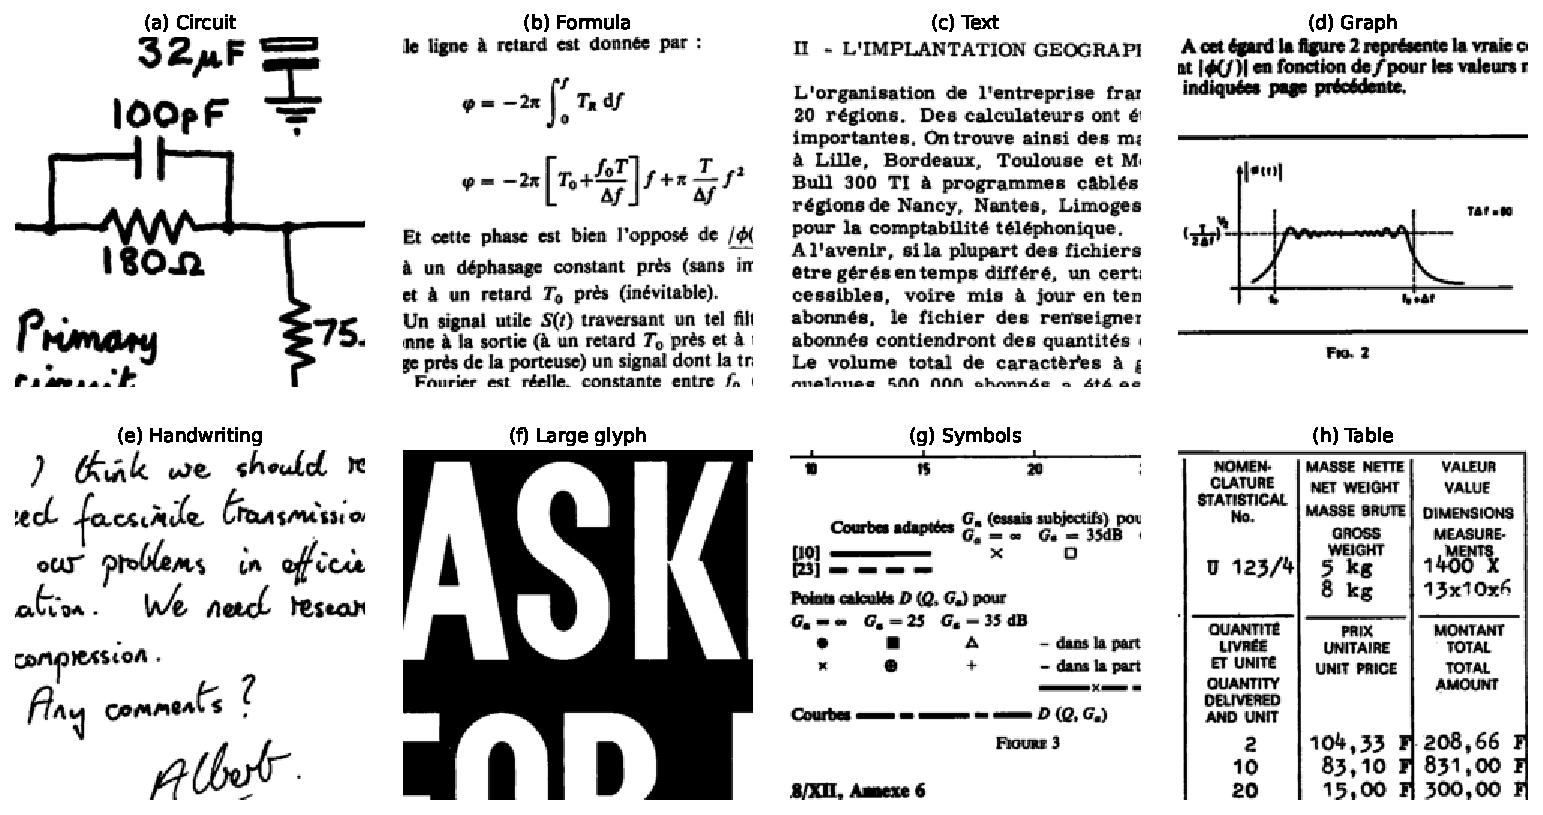
\includegraphics[width=\textwidth]{images/Figure_4.pdf}
\caption{Eight binary document images used for block-mapping validation.}
\label{fig:dataset-final}
\end{figure*}

\RevisionAddBegin
The four-method BOSSbase protocol embeds identical pseudorandom messages at
targets 64, 128, 256, and 512 bits. A run counts as available after exact
message extraction and bitwise cover restoration. Huynh--Nguyen uses the
published threshold $T=5$. Dong evaluates all context divisors
$l\in\{1,\ldots,10\}$ and retains the exact minimum-DRD result. PPOCP and Dong
use conservative serialized synchronization or location information where the
publications leave the independent wire representation open. Accordingly,
net-payload conclusions apply to the executable wire formats defined in this
study, while DRD and availability provide a comparison less sensitive to
byte-stream conventions.

The FUNSD protocol is deliberately narrower and tests transfer rather than a
new four-method ranking. At each target $q\in\{64,128,256,512\}$, it compares
A1, which activates all feasible tables and then charges their exact wire cost,
with the proposed A2 serialization-aware prefix selection. The same frozen CNN
weights and seed 20260608 are used throughout. Availability, auxiliary bits,
delivered net payload, DRD, positive-net fraction, and exact message/cover
round-trip recovery are recorded per image; paired A1/A2 summaries are computed
only where both variants are available.

\RevisionAddEnd

\subsection{Metrics and Statistical Protocol}

